Mivel a dolgozatban bemutatott szoftver azt a célt szolgálja, hogy egy esetleges vásárló reális képet alkosson egy termék árának változásáról, ezért ebben a fejezetben a használat során történt észrevételek lesznek bemutatva, tanulmányozva. A tanulmány a legnagyobb Romániai online áruházra fog koncentrálni, mely jelen pillanatban az Emag, ugyanakkor nagyító alá kerülnek a 2020-as Black Friday alatt történt észrevételek és események is. 

Mivel nagyon sokszor hallottunk olyan történeteket, melyekben az emberek hamis árakról vagy promóciókról panaszkodtak, ezért a fejlesztett szoftvert felhasználva, követtünk pár népszerű terméket, melyeket egy átlag felhasználó megvásárolna, ilyenek például pár mobil telefon, úgy felső, mint közép kategóriából, az árukat tekintve, laptopok és egyéb elektronikai eszközök, de pár parfüm is helyet kapott. Az észrevételek esetenként több hónapnyi adatókból lettek megfogalmazva, viszont ezek közül néhány kifejezetten a népszerű Black Friday periódusra koncentrálódik. 

A legsűrűbbén észrevett minta, amely szinte minden termék esetében megjelenik, az a hirtelen ár növekedés, mely egy napig vagy sok esetben csak fél napig van jelen. Ilyenkor úgy tűnik mintha a kereskedő megpróbálná úgymond drágábban eladni a terméket, vagyis teszteli a piacot. Megfigyelhető az is, hogy egy pár ilyen hirtelen növekedés után, egy kis idő elteltével stabilizálódik a termék ára sokszor egy magasabb értéken, majd onnan megint következik az újabb időnkénti növekedés. Mindez a \ref{fig:spikes} ábrán látható is.

\begin{figure}[H]
    \centering
    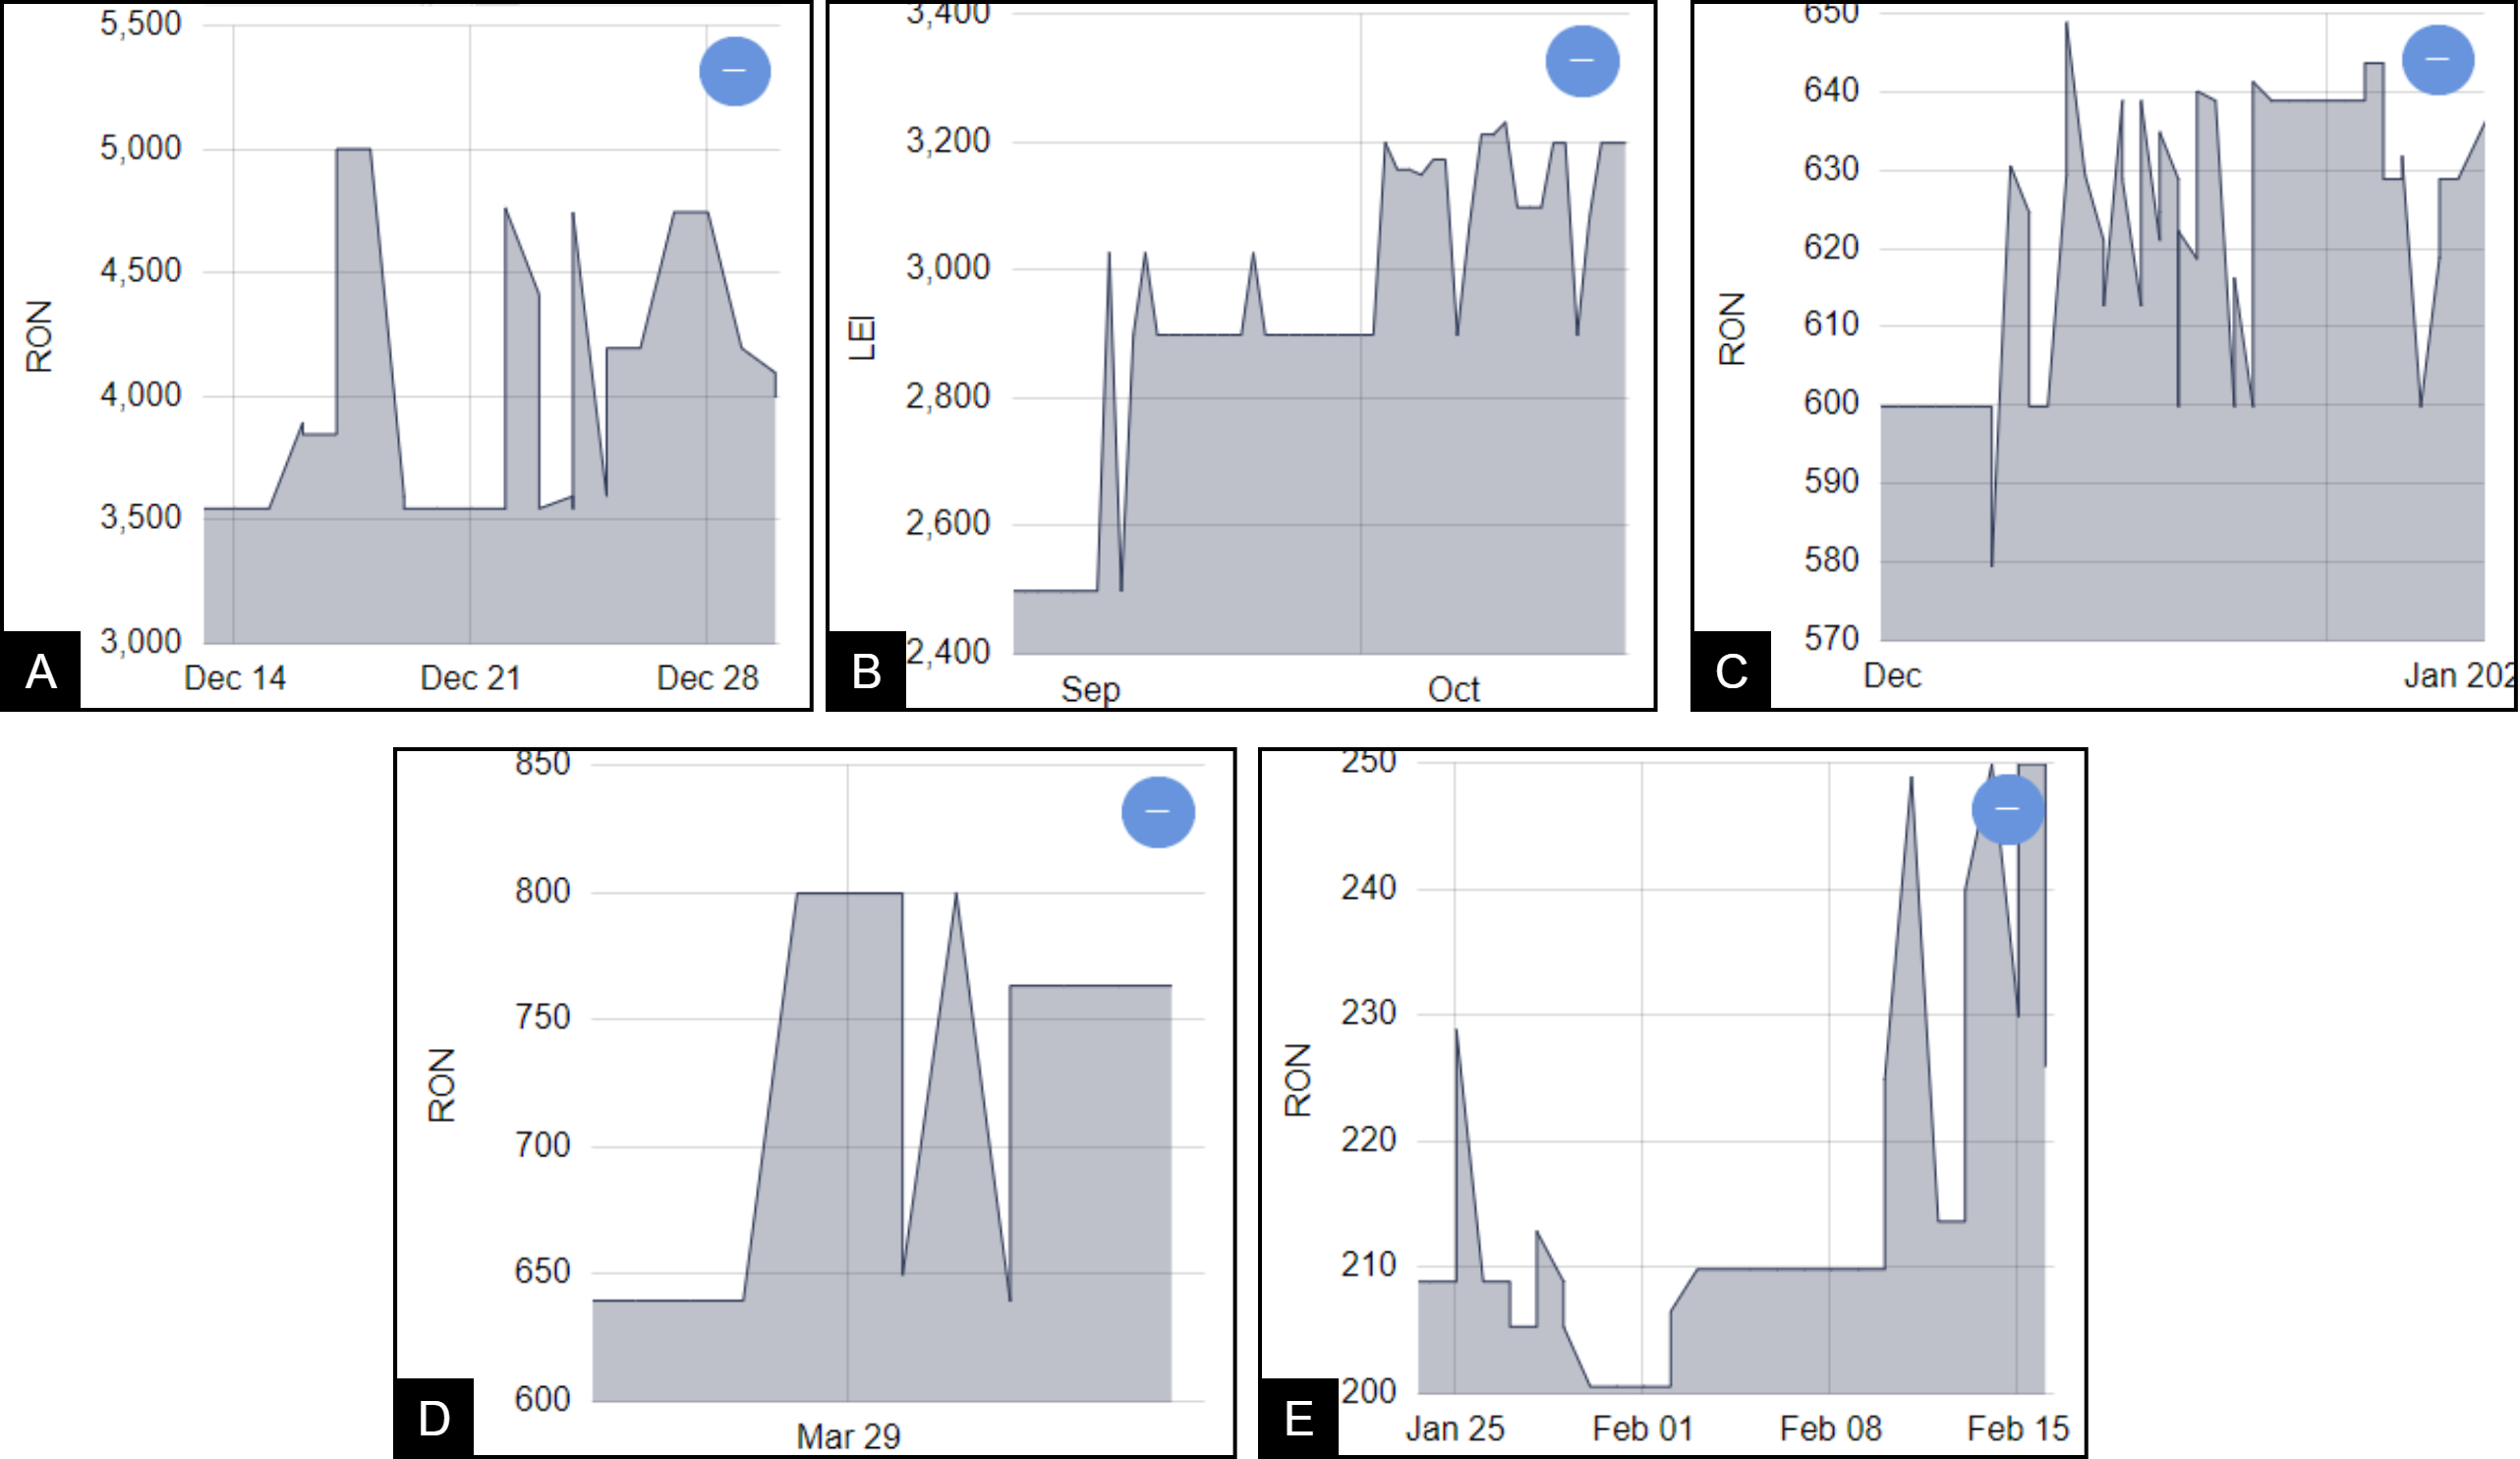
\includegraphics[scale=1]{figures/images/study/spikes.png}
    \caption{Megfigyelt időszakos árnövekedések különböző termékek esetében}
    \label{fig:spikes}
\end{figure}

A - iPhone 11 - \url{https://tinyurl.com/5xa8y7u7} 
% \url{https://www.emag.ro/telefon-mobil-apple-iphone-11-128gb-black-mwm02rm-a/pd/DF9ZX6BBM/?ref=fam\#128-GB}

B - Huawei Matebook laptop - \url{https://tinyurl.com/yw99mcdp}
% \url{https://www.emag.ro/laptop-huawei-matebook-d15-2020-cu-procesor-amd-ryzentm-5-3500u-pana-la-3-70-ghz-15-6-full-hd-ips-8gb-256gb-ssd-radeontm-vega-8-windows-10-home-mystic-silver-53010uaj/pd/DR0S1BMBM/?ref=prod_CMP-62795_5755_66183}

C - Samsung Galasy A20e - \url{https://tinyurl.com/2v9hdj68}
% \url{https://www.emag.ro/telefon-mobil-samsung-galaxy-a20e-dual-sim-32gb-4g-blue-sm-a202fzbdrom/pd/D4WMHQBBM/?ref=graph_profiled_similar_a_1_4&provider=rec&recid=rec_49_16_c2732421_93_A_abf22371c7da6b38789077ed715b15f41a6dcdf024ef601701a96e1359be610a_1603731413&scenario_ID=49}

D - Xiaomi Poco M3 - \url{https://tinyurl.com/2kp3ezxk}
% \url{https://www.emag.ro/telefon-mobil-poco-m3-dual-sim-64gb-4g-cool-blue-poco-m3-64-blue/pd/DFRJR7MBM/?ref=fam\#Albastru}

E - Samsung Galaxy Fit 2 smartband - \url{https://tinyurl.com/dnz6b7pc}
% \url{https://www.emag.ro/bratara-fitness-samsung-galaxy-fit-2-black-sm-r220nzkaeue/pd/DY3YH2MBM/}

\section{Black Friday}

Mivel a szoftver létrejöttet nagyban inspirálta a Black Friday-kor történő manipulálások, ezért egy pár észrevétel ehhez kötődően is bemutatásra kerül. Romániában a Black Friday 2020-ban November 13 rendeződött meg. Annak köszönhetően, hogy rengeteg termék található az Emag online áruházában, ezért nehéz általánosítani és azt mondani, hogy minden termék hamis leszállítással vagy promócióval rendelkezik, viszont ezek elfőfordulnak. Ezért a következőkben egy pár általunk észlelt jelentős és érdekes eset lesz bemutatva.

Első esetben egy parfüm árának figyelésekor tettük meg azt az észrevételt, hogy a termék ára egy nappal a Black Friday időpontja elött, megnőtt az előző napokhoz képest. Eddig semmi meglepő nem történt, hiszen erre számítottunk is sok termék esetében, viszont ebben az esetben az érdekességet az képviselte, hogy a termék drágább lett, de az esemény napján várt esés nem történt meg, pedig a szóban forgó parfüm akciósként volt megjelölve (\ref{fig:parfum} ábra). Egy másik termék esetében, mely szintén egy parfüm volt, ugyanez a jelenség játszódott le, a termék drágább volt az esemény napján, az azelőtti árához képest, viszont, ugyanez a termék ugyanaz nap egy esti órájában még a reggeli árat is meghaladta, mindeközben egyre nagyobb árleszállítást reklámozva. Tehát az árleszállítás mértéke nagyobb lett, viszont a termék drágult.

\begin{figure}[H]
    \centering
    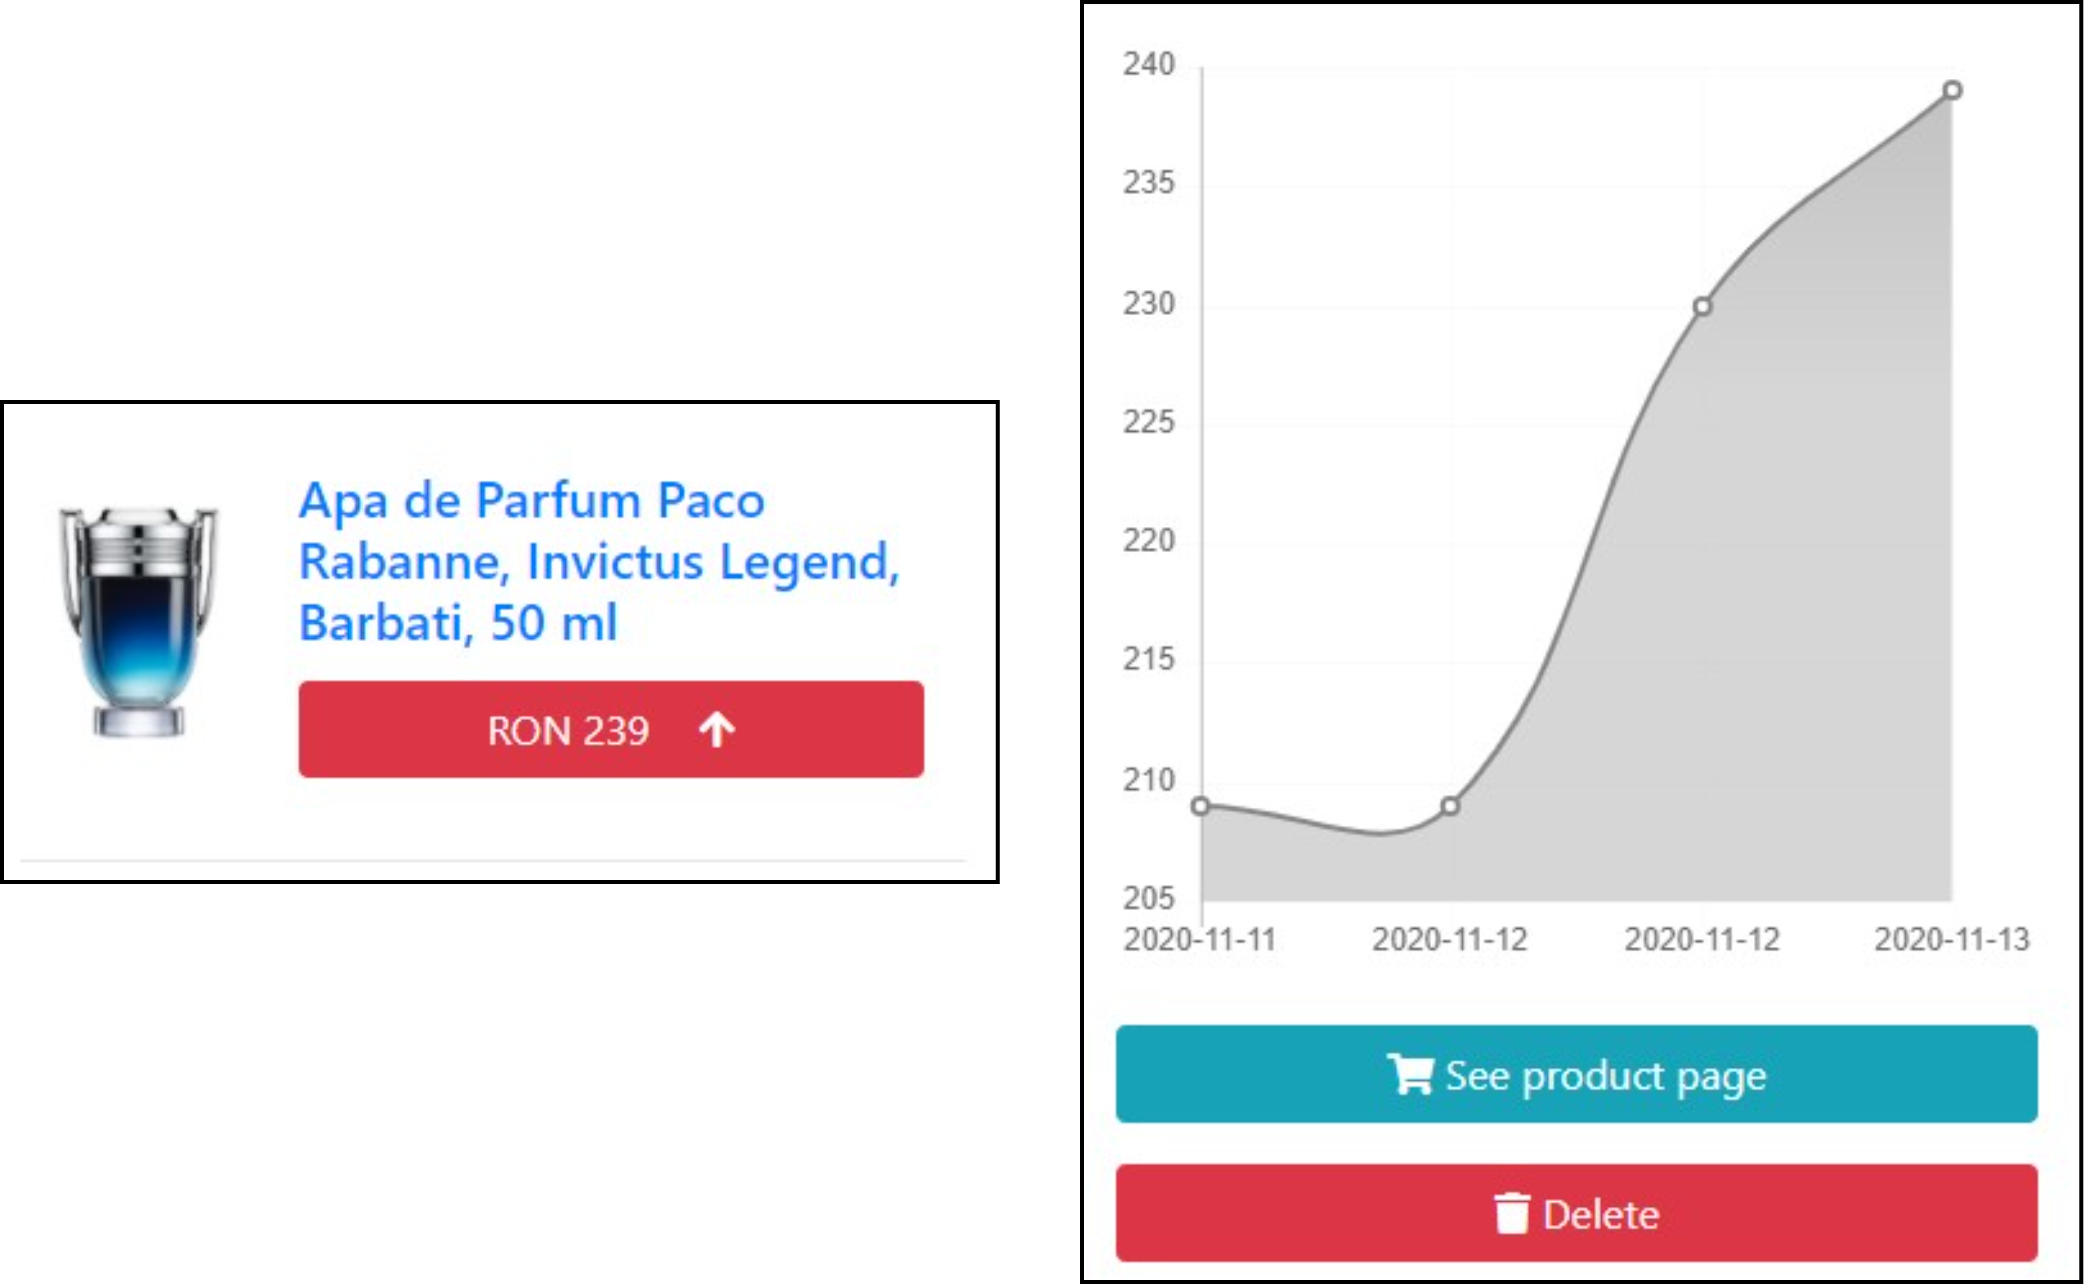
\includegraphics[scale=0.9]{figures/images/study/parfum.png}
    \caption{Példa az ár növekedésére már Black Friday elött}
    \label{fig:parfum}
\end{figure}

Egy másik érdekes észrevétel ugyanilyen formában fogalmazódott meg, több termék árának többszöri változásával a nap folyamán, de ezekben az esetekben, ezek reális csökkenések voltak. Ezek a bizonyos észrevételek telefonok követésekor voltak megfigyelve, amik esetében tényleg jóval alacsonyabb volt az akciósként megjelölt ár, az előző időszakhoz képest. Mivel az előző esetben tárgyalt többszöri változást láttuk már, ezekben az estekben a leírt jelenség fordítottja történt. Vagyis az esemény napján, a termék ára kétszer is csökkent, mindkétszer reálisan (\ref{fig:real_sale} ábra).

\begin{figure}[H]
    \centering
    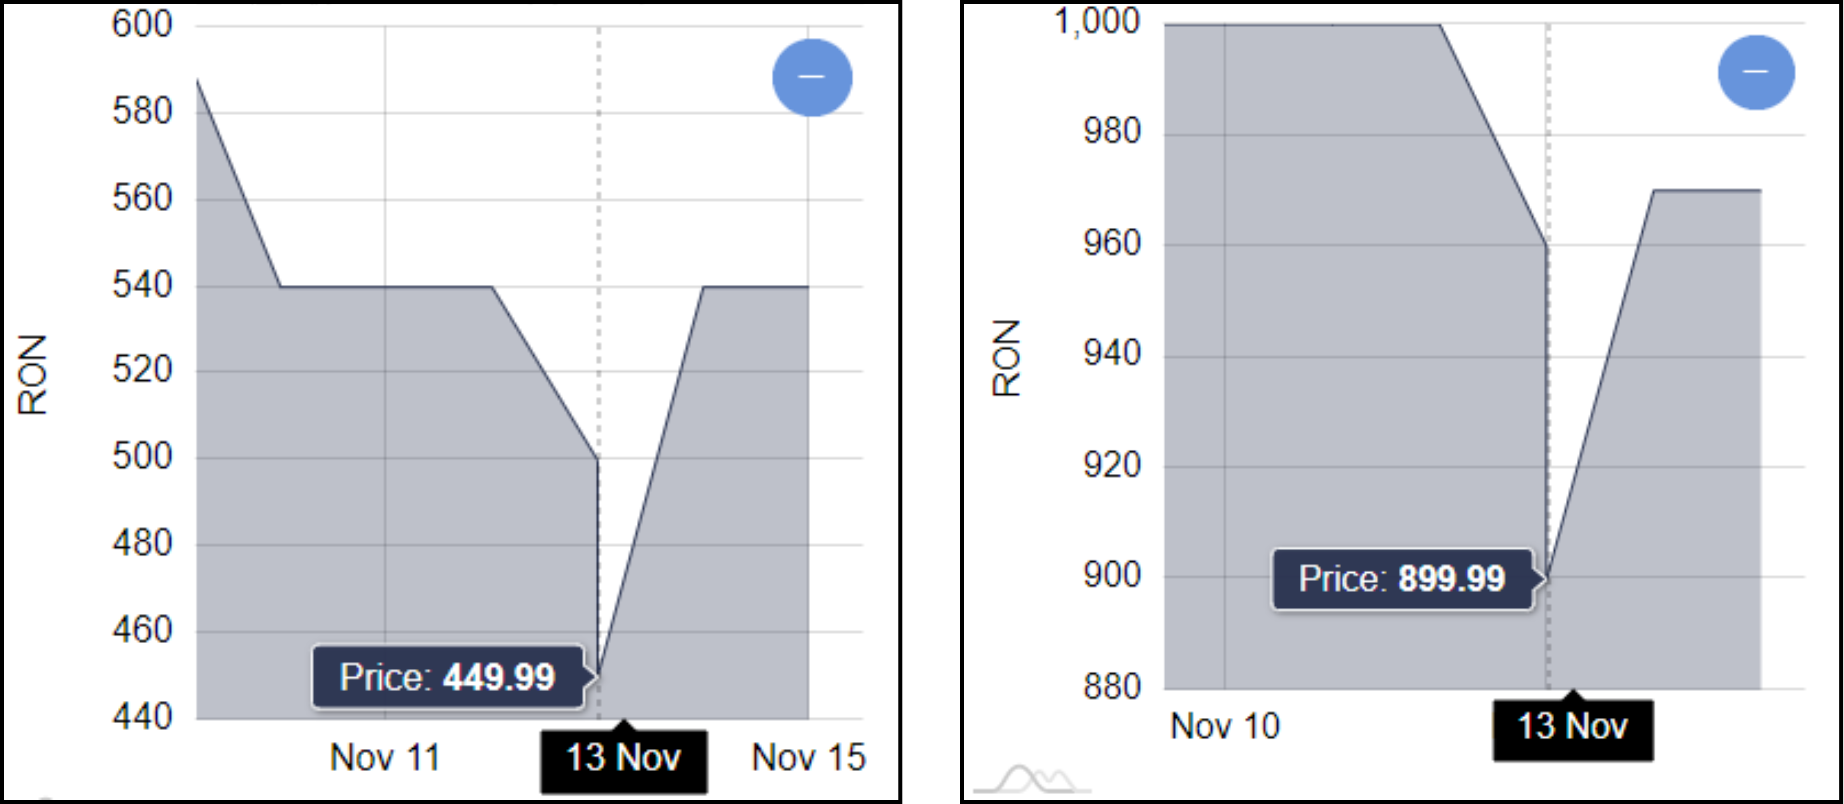
\includegraphics[scale=1]{figures/images/study/real_sale.png}
    \caption{Többszörös árcsökkentés Black Friday napján}
    \label{fig:real_sale}
\end{figure}

Mivel a laptopok az egyik legnépszerűbb termékek voltak idén ősszel, a kialakult vírus helyzet miatt otthonról dolgozók, illetve tanulók köreiben, természetesen ezek sem maradhattak el a várt kedvezményektől legalábbis a látszólagosaktól. Az akkoriban rendelkezésre álló adathalmazban csupán egyetlen laptop volt jelen, amire érvényes volt az esemény elött pár nappal való ár növekedés (\ref{fig:laptop}).
\begin{figure}[H]
    \centering
    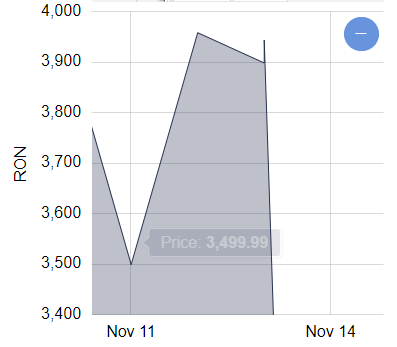
\includegraphics[scale=0.8]{figures/images/study/laptop_blackfriday.png}
    \caption{Laptop mesterséges árleszállítása}
    \label{fig:laptop}
\end{figure}